% Source for the figure of convexHull() (sec. 16.2): 58 random points, the
% octagon of their extreme points in the eight directions (shaded; here 7
% distinct vertices), the points strictly inside it, which the filter drops
% (grey), the ones it keeps (black), and the hull (dashed). Written by a
% script that applies the rules of ConvexHull.tpp. Build: make figures (in
% ../build).
\documentclass[border=4pt]{standalone}
\usepackage[T1]{fontenc}
\usepackage{newpxtext,newpxmath}
\usepackage[varqu,varl,scaled=0.95]{zi4}
\usepackage{tikz}
% tikz-ads.tex: the TikZ styles shared by the figures of the memory of the
% manual, \input by each standalone figure: a cell of a vector (cell), the
% cell that an operation touches (touched), a free cell (free), a node of a
% linked structure (node), the labels of indices (index) and of variables
% (var), a pointer (ptr), and \cells and \indices to draw a row of cells.
\usetikzlibrary{arrows.meta,positioning,calc,fit,shapes.multipart}
\definecolor{adsTouched}{RGB}{214,196,236}
\definecolor{adsFree}{RGB}{236,236,236}
\tikzset{
  ads/.style={>={Stealth[length=2mm]},font=\small,
              every node/.append style={inner sep=0pt}},
  cell/.style={draw,minimum width=7mm,minimum height=7mm,
               font=\small\ttfamily,outer sep=0pt},
  touched/.style={cell,fill=adsTouched},
  free/.style={cell,fill=adsFree,text=black!45},
  node/.style={draw,rounded corners=1pt,minimum width=8mm,
               minimum height=6mm,font=\small\ttfamily},
  index/.style={font=\scriptsize\ttfamily,text=black!60},
  var/.style={font=\small\itshape},
  ptr/.style={->,thick}
}
% \cells{name}{x,y}{list}: a row of cells, the first at (x,y), named
% name-0, name-1, ...; each item is text/style, the style one of cell,
% touched and free (e.g., {a/cell,e/touched,/free})
\newcommand{\cells}[3]{%
  \foreach \v/\s [count=\i from 0] in {#3}
    \node[\s] (#1-\i) at ($(#2)+(\i*7mm,0)$) {\v};}
% \indices{name}{n}: the indices 0 .. n-1 under the cells of name
\newcommand{\indices}[2]{%
  \foreach \i in {0,...,\numexpr#2-1\relax}
    \node[index,below=1.2mm of #1-\i] {\i};}

\tikzset{
  ext/.style={rectangle,fill=black,minimum size=2mm},
  kept/.style={circle,fill=black,minimum size=1.5mm},
  drop/.style={circle,draw=black!45,fill=adsFree,minimum size=1.3mm}
}
\begin{document}
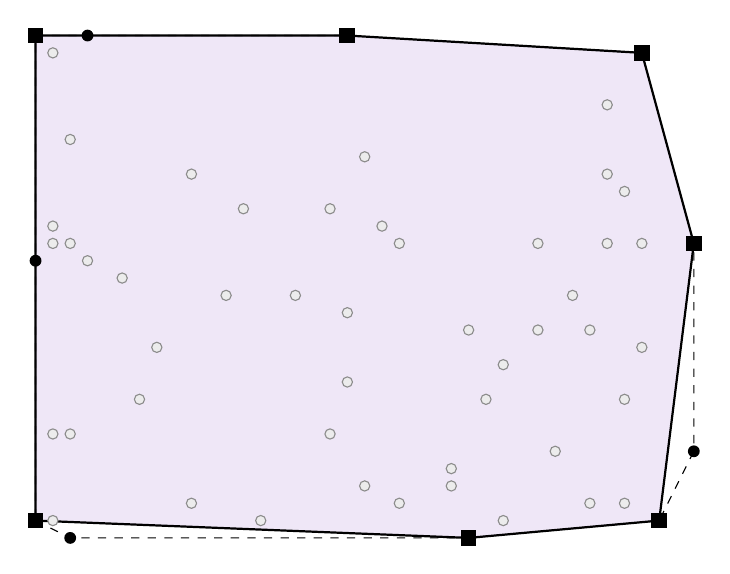
\begin{tikzpicture}[ads,x=2.2mm,y=2.2mm]
  \draw[thick,fill=adsTouched!40] (27,1) -- (38,2) -- (40,18) -- (37,29) -- (20,30) -- (2,30) -- (2,2) -- cycle;
  \draw[dashed] (2,2) -- (4,1) -- (27,1) -- (38,2) -- (40,6) -- (40,18) -- (37,29) -- (20,30) -- (2,30) -- cycle;
  \node[ext] at (20,30) {};
  \node[drop] at (9,12) {};
  \node[drop] at (3,2) {};
  \node[drop] at (34,3) {};
  \node[drop] at (23,18) {};
  \node[drop] at (3,29) {};
  \node[drop] at (32,6) {};
  \node[ext] at (2,2) {};
  \node[drop] at (27,13) {};
  \node[drop] at (4,7) {};
  \node[drop] at (5,17) {};
  \node[ext] at (27,1) {};
  \node[drop] at (36,3) {};
  \node[drop] at (14,20) {};
  \node[ext] at (40,18) {};
  \node[drop] at (3,18) {};
  \node[drop] at (37,12) {};
  \node[drop] at (3,7) {};
  \node[kept] at (2,17) {};
  \node[drop] at (8,9) {};
  \node[drop] at (26,4) {};
  \node[drop] at (36,9) {};
  \node[drop] at (35,26) {};
  \node[drop] at (11,3) {};
  \node[drop] at (37,18) {};
  \node[kept] at (40,6) {};
  \node[drop] at (23,3) {};
  \node[drop] at (35,22) {};
  \node[drop] at (4,18) {};
  \node[drop] at (3,19) {};
  \node[drop] at (13,15) {};
  \node[drop] at (34,13) {};
  \node[drop] at (20,14) {};
  \node[ext] at (37,29) {};
  \node[drop] at (29,11) {};
  \node[drop] at (19,7) {};
  \node[drop] at (11,22) {};
  \node[drop] at (15,2) {};
  \node[drop] at (33,15) {};
  \node[drop] at (21,23) {};
  \node[drop] at (28,9) {};
  \node[ext] at (38,2) {};
  \node[drop] at (7,16) {};
  \node[drop] at (26,5) {};
  \node[drop] at (21,4) {};
  \node[drop] at (31,13) {};
  \node[ext] at (2,30) {};
  \node[drop] at (4,24) {};
  \node[drop] at (35,18) {};
  \node[drop] at (20,10) {};
  \node[drop] at (22,19) {};
  \node[drop] at (31,18) {};
  \node[drop] at (29,2) {};
  \node[kept] at (5,30) {};
  \node[drop] at (17,15) {};
  \node[kept] at (4,1) {};
  \node[drop] at (19,20) {};
  \node[drop] at (36,21) {};\end{tikzpicture}
\end{document}
